\documentclass[10pt,a5]{article}

\usepackage{paracol}
%\usepackage[landscape]{geometry}
\usepackage[left=1.5cm, right=1.5cm, top = 2cm, bottom = 2cm]{geometry}
%\usepackage{pdfpages}
\usepackage{graphicx}
\usepackage{liturg}
\usepackage{lipsum}

\newcommand \sect[2] {\section*{#1} \switchcolumn \section*{#2} \switchcolumn*}
\newcommand \subsect[2] {\subsection*{#1} \switchcolumn \subsection*{#2} \switchcolumn*}

\begin{document}

\massenglish

%\psalmheading{Psalm 42---Judica me}

%\instruct{The priest, signing himself with the Sign of the Cross, says:}

%\leslettrine{C}onf'iteor Deo omnipot'enti, be'at"ae Mar'i"ae semper
%V'irgini, be'ato Micha'eli Arch'angelo, be'ato Jo'anni Bapt'ist"ae,
%sanctis Ap'ostolis Petro et Paulo, 'omnibus Sanctis, et tibi Pater:
%quia pecc'avi nimis congitati'one, verbo, et 'opere:

\begin{paracol}{2}

\sect{Introductory Rites}{Ritos Iniciais}

\subsect{Entrance}{Canto de Entrada}

\subsect{Greeting}{Acolhida}

\switchcolumn

\priest{The Lord be with you}

\server{And with your spirit}

\switchcolumn

\padre{A graça de Nosso Senhor Jesus Cristo, o amor do Pai e a comunhão do Espírito Santo estejam convosco.}
\todos{Bendito seja Deus, que nos reuniu no amor de Cristo.}

\switchcolumn*

\subsect{Penitential Act}{Ato Penitencial}

\end{paracol}

\begin{figure}[h]
	\centering
	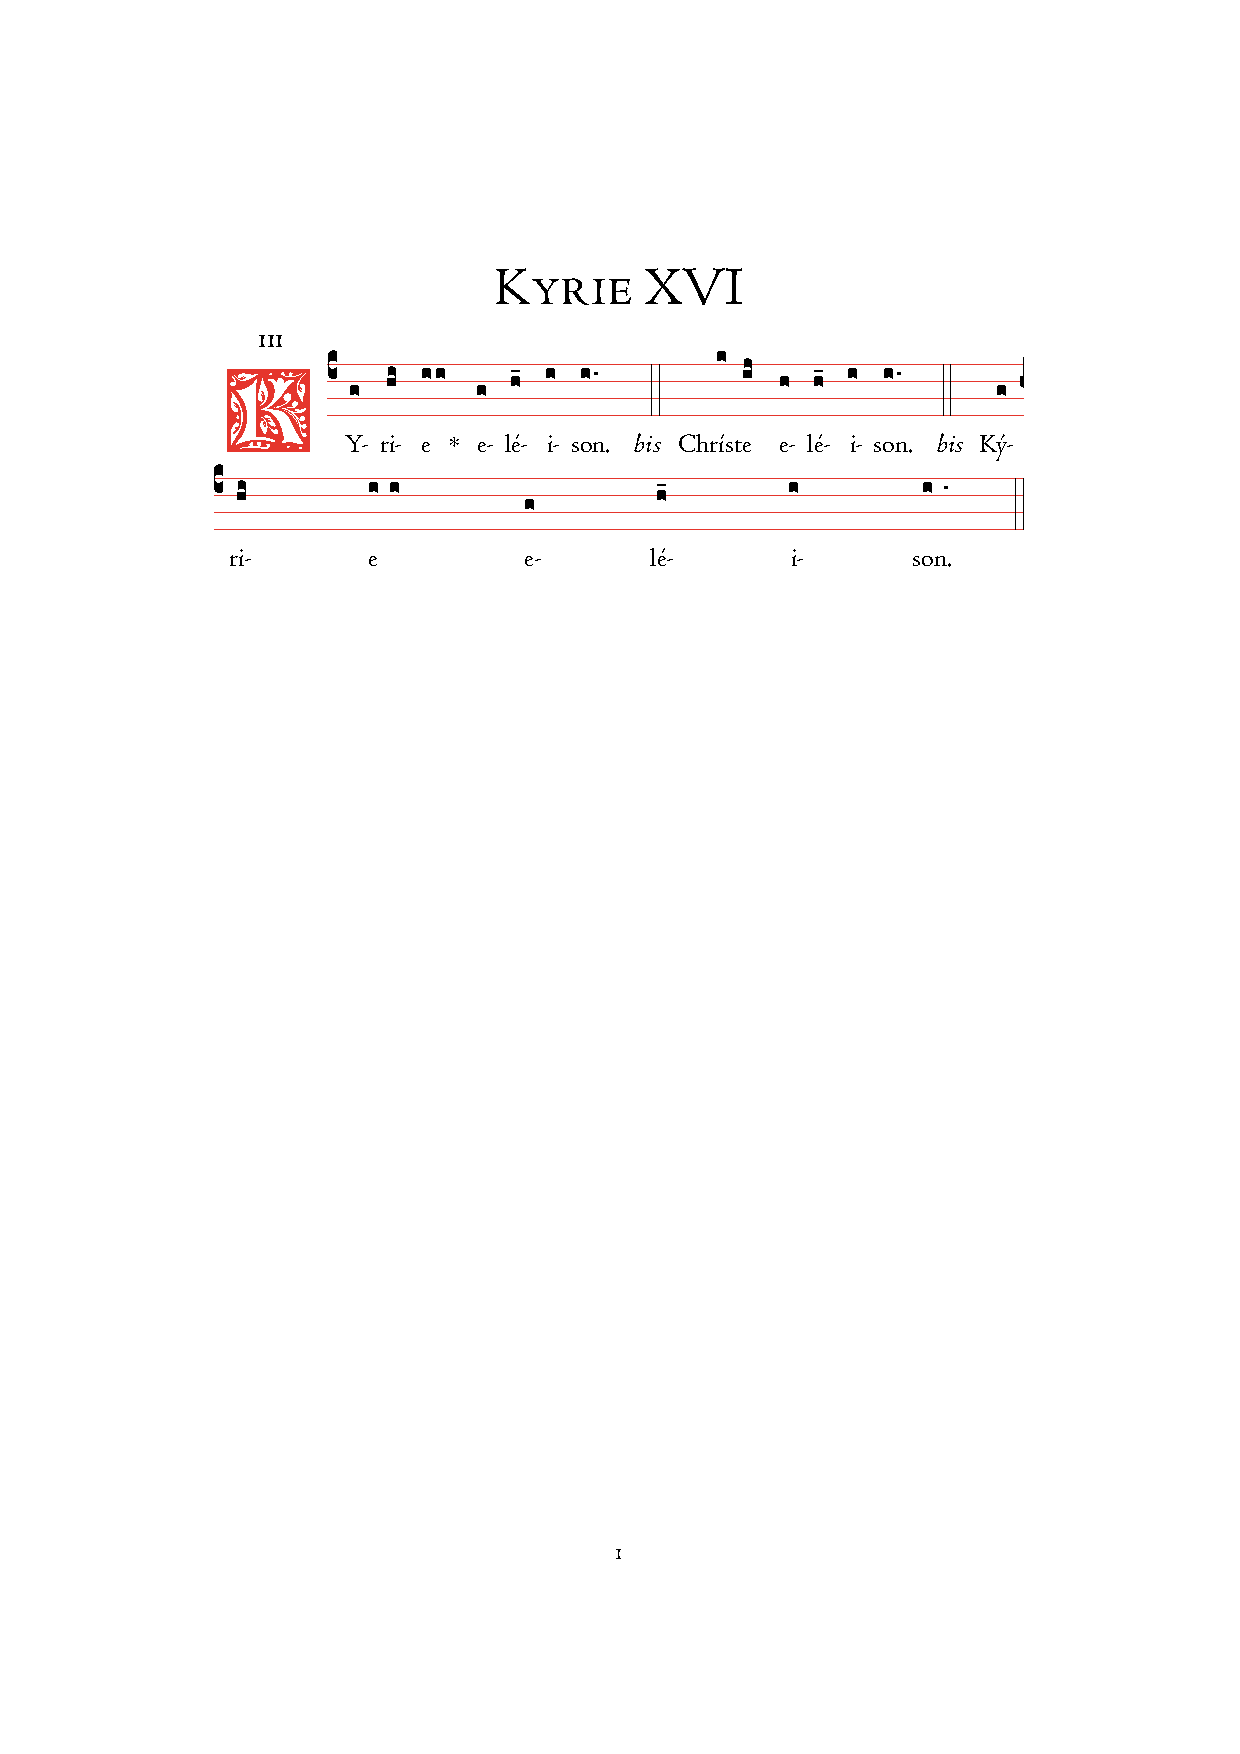
\includegraphics[trim = 35mm 200mm 35.5mm 45mm, clip, width = 0.8\textwidth]{scores/Kyrie-XVI.pdf}
\end{figure}

\begin{paracol}{2}

(Lord, have mercy. Christ, have mercy. Lord, have mercy.)
\switchcolumn
(Senhor, tende piede. Cristo, tende piedade. Senhor, tende piedade)

\switchcolumn*

\subsect{Glory to God}{Gl\'oria}

\end{paracol}

\begin{figure}
	\centering
	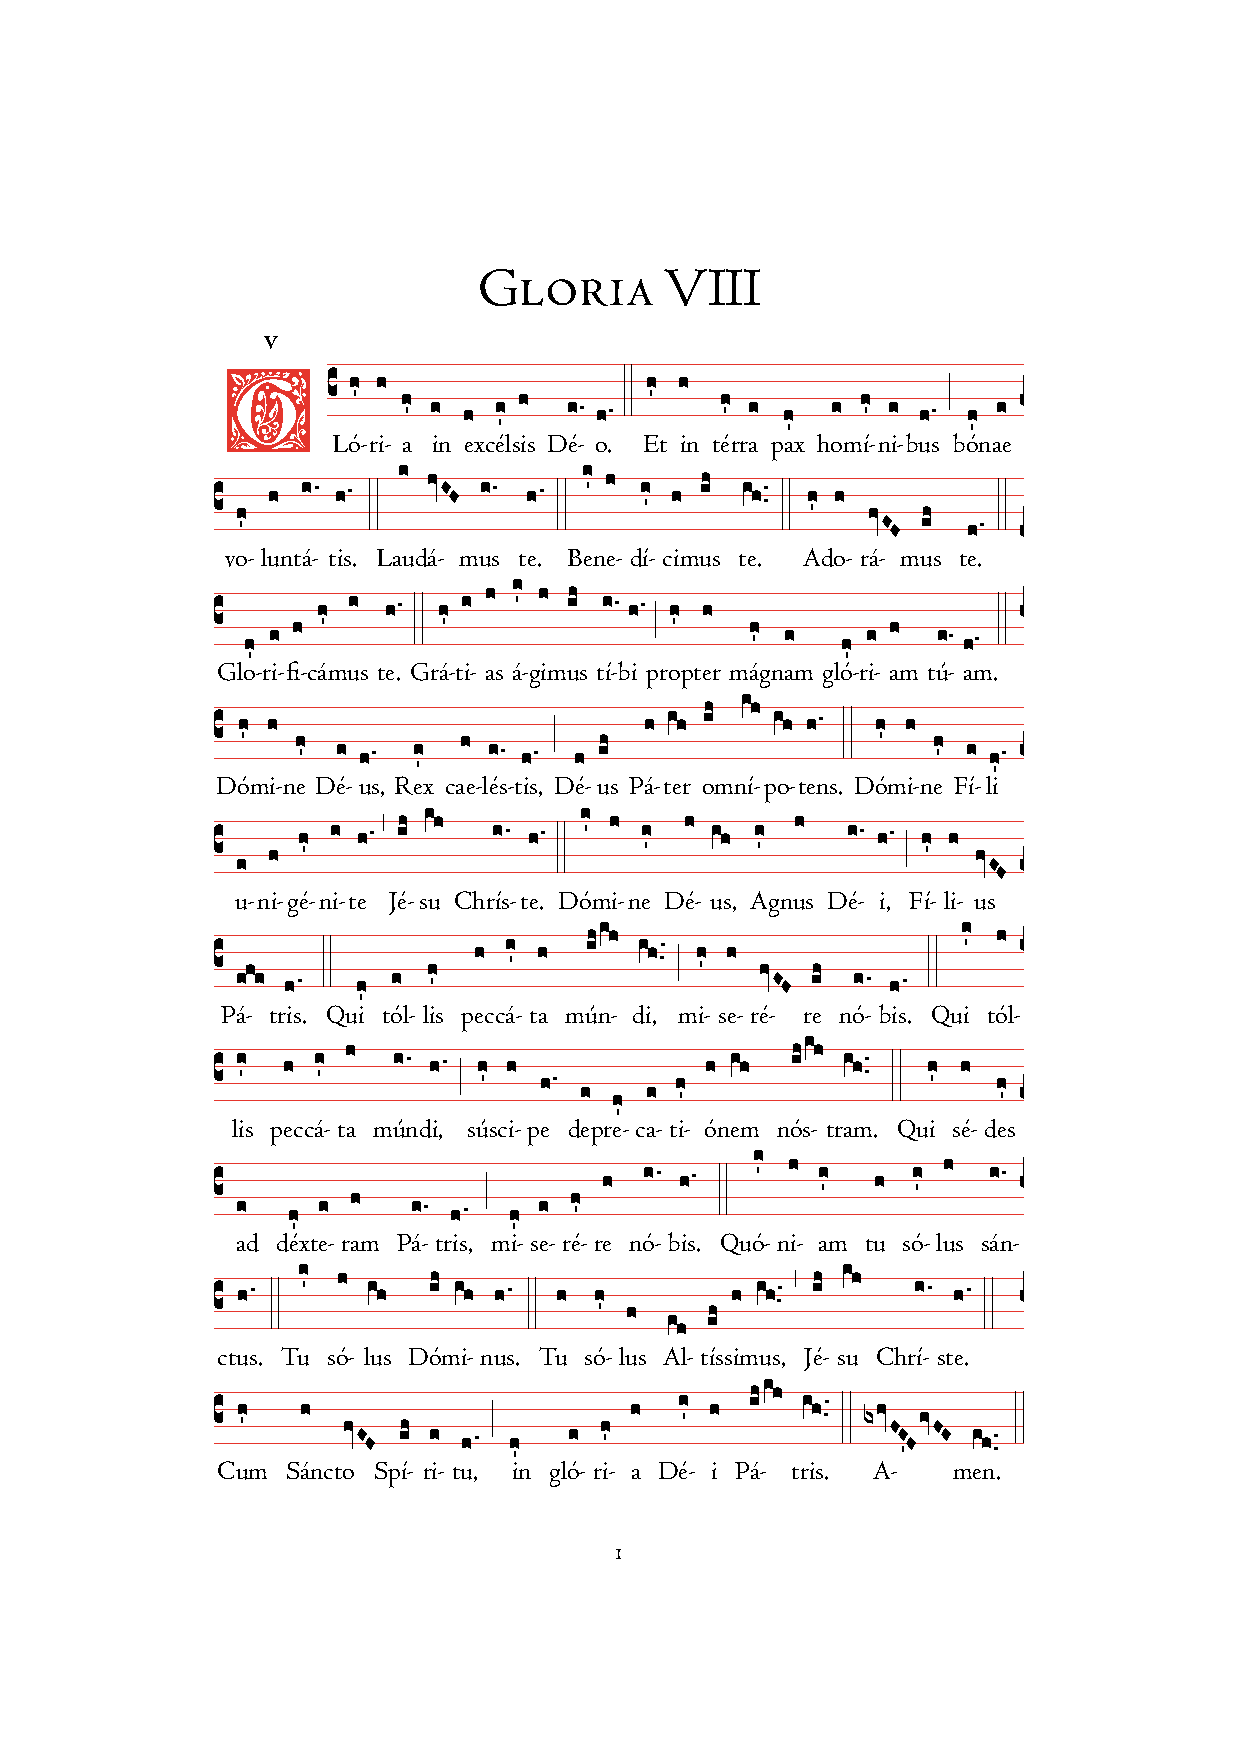
\includegraphics[trim = 35mm 45mm 35.5mm 45mm, clip, width = 0.8\textwidth]{scores/Gloria-VIII.pdf}
\end{figure}

\begin{paracol}{2}

(Glory to God in the highest,
and on earth peace to people
of good will.
We praise you, we bless you,
we adore you, we glorify you,
we give you thanks for your great
glory,
Lord God, heavenly King, O God,
almighty Father.
Lord Jesus Christ, Only Begotten Son,
Lord God, Lamb of God, Son of the
Father,
you take away the sins of the world,
have mercy on us;
you take away the sins of the world,
receive our prayer;
you are seated at the right hand
of the Father, have mercy on us.
For you alone are the Holy One,
you alone are the Lord,
you alone are the Most High,
Jesus Christ, with the Holy Spirit,
in the glory of God the Father. Amen.)

\switchcolumn

(Gl\'oria a Deus nas alturas e paz na terra aos homens por Ele amados.
 Senhor Deus, Rei dos c\'eus, Deus Pai todo-poderoso:
 n\'os Vos louvamos, n\'os Vos bendizemos, n\'os Vos adoramos, n\'os Vos glorificamos,
 n\'os Vos damos graças, por vossa imensa gl\'oria.
 Senhor Jesus Cristo, Filho Unig\'enito, Senhor Deus, Cordeiro de Deus, Filho de Deus Pai:
 V\'os que tirais o pecado do mundo, tende piedade de n\'os;
 V\'os que tirais o pecado do mundo, acolhei a nossa s\'uplica;
 V\'os que estais \`a direita do Pai, tende piedade de n\'os.
 S\'o V\'os sois o Santo;
 s\'o V\'os, o Senhor;
 s\'o V\'os, o Alt\'issimo, Jesus Cristo;
 com o Esp\'irito Santo na gl\'oria de Deus Pai.
 Am\'em)

 \switchcolumn*

 \sect{Litugy of the Word}{Liturgia da Palavra}

 \sect{First Reading}{Primeira Leitura}

 \lipsum[3]

 \server{Thanks be to God!}

 \switchcolumn

 \lipsum[3]

 \todos{Gra\c{c}as a Deus!}

 \switchcolumn*

 \subsect{Responsorial Psalm}{Salmo Responsorial}

 \lipsum[1]

 \switchcolumn

 \lipsum[1]

 \switchcolumn*

 \subsect{Second Reading}{Segunda Leitura}

 \lipsum[3]

 \server{Thanks be to God.}

 \switchcolumn

 \lipsum[3]

 \todos{Gra\c{c}as a Deus!}

 \switchcolumn*

 \subsect{Gospel}{Evangelho}

 \lipsum[3]

 \server{Glory to you O Lord.}

 \switchcolumn

 \lipsum[3]

 \todos{Gl\'oria a v\'os, Senhor!}

 \switchcolumn*

 \subsect{Homily}{Homilia}

 \subsect{The Creed}{Profiss\~ao de f\'e}
I believe in one God,
the Father almighty,
maker of heaven and earth,
of all things visible and invisible.
I believe in one Lord Jesus Christ,
the Only Begotten Son of God,
born of the Father before all ages.
God from God, Light from Light,
true God from true God,
begotten, not made,
consubstantial with the Father;
through him all things were made.
For us men and for our salvation
he came down from heaven,
At the words that follow, up to and including and became
man, all bow.
and by the Holy Spirit was incarnate
of the Virgin Mary,
and became man.
For our sake he was crucified
under Pontius Pilate,
he suffered death and was buried,
and rose again on the third day
in accordance with the Scriptures.
He ascended into heaven
and is seated at the right hand
of the Father.
He will come again in glory
to judge the living and the dead
and his kingdom will have no end.
I believe in the Holy Spirit,
the Lord, the giver of life,
who proceeds from the Father
and the Son,
who with the Father and the Son
is adored and glorified,
who has spoken through the prophets.
I believe in one, holy, catholic
and apostolic Church.
I confess one Baptism
for the forgiveness of sins
and I look forward to the resurrection
of the dead
and the life of the world to come. Amen.
The Apostles’ Creed
I believe in God,
the Father almighty,
Creator of heaven and earth,
and in Jesus Christ, his only Son,
our Lord,
{\tiny At the words that follow, up to and including the Virgin Mary, all bow.}
who was conceived by the Holy Spirit,
born of the Virgin Mary,
suffered under Pontius Pilate,
was crucified, died and was buried;
he descended into hell;
on the third day he rose again
from the dead;
he ascended into heaven,
and is seated at the right hand
of God the Father almighty;
from there he will come to judge
the living and the dead.
I believe in the Holy Spirit,
the holy catholic Church,
the communion of saints,
the forgiveness of sins,
the resurrection of the body,
and life everlasting. Amen.

\end{paracol}

%\greatfeast{Feria Quinta in Cena Domini}{I}

%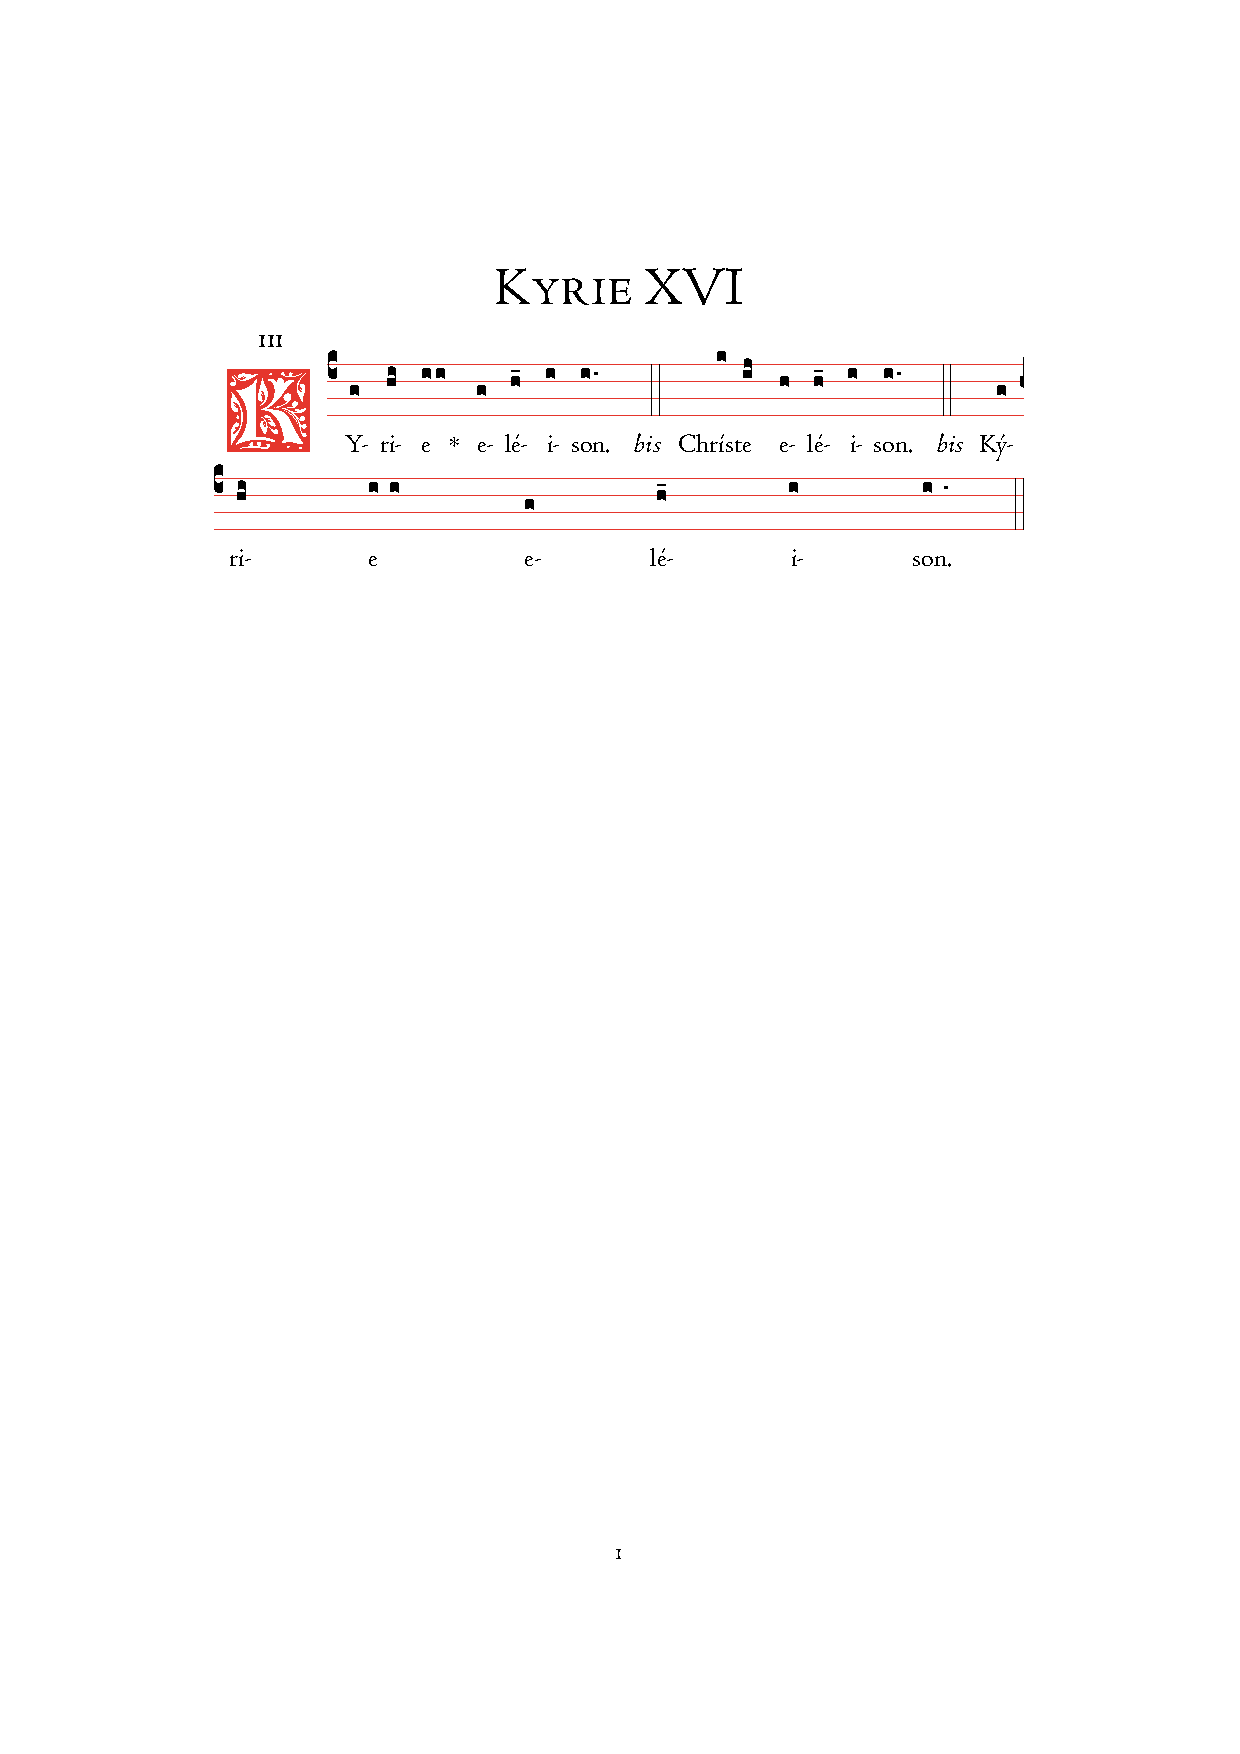
\includepdf[pages=-,pagecommand={},width=\textwidth, trim = 35mm 200mm 20mm 45mm, clip]{scores/Kyrie-XVI.pdf}
\end{document}
